% !TeX program = lualatex
\documentclass[aspectratio=169, xcolor=dvipsnames, t]{beamer}

\RequirePackage[british]{babel}  % Sprache
\RequirePackage{csquotes}  % Anführungszeichen

\RequirePackage{geometry}  % Seitenlayout (insbesondere Ränder)

\RequirePackage{amsmath, amssymb, amsthm}  % mathematische Grundlagen
\let\mathbbold\mathbb  % speichere herkömmliche Buchstaben mit Doppelstrich und Serifen
\RequirePackage[intlimits]{mathtools}  % stellt u. a. \DeclarePairedDelimiter zur Verfügung + weitere Verbesserungen für amsmath
\RequirePackage[math-style=ISO, bold-style=ISO, partial=upright]{unicode-math}  % für kursive gr. Großbuchstaben und aufrechtes ∂ benützt
\let\mathbb\mathbbold  % kehre zu herkömmlichen Buchstaben mit Doppelstrich und Serifen zurück; neue Zeichen wie 1 mittels \symbb{1} verfügbar
\RequirePackage{xfrac}  % schräge Brüche; vor fontspec zu laden!

\RequirePackage[protrusion=true]{microtype}  % für hängende Interpunktion
\RequirePackage{tabularx}  % bessere Trenner und Zeilentypen
\makeatletter
\@ifclassloaded{beamer}{}{\RequirePackage[inline]{enumitem}}  % bessere Aufzählung (mit *-Variante für Aufzählungen innerhalb eines Textes); für 'beamer' ausgeschaltet
\makeatother

\PassOptionsToPackage{dvipsnames}{xcolor}
\RequirePackage{tikz} % Grafikpaket
\RequirePackage{tikzpagenodes}  % benötig für current page
\RequirePackage{pgfplots}  % tikz-Erweiterung
\pgfplotsset{compat=1.18}

\RequirePackage[ruled, lined, longend, nofillcomment, linesnumbered]{algorithm2e}

\RequirePackage{hyperref}  % klickbare Verweise
\RequirePackage[nameinlink, noabbrev]{cleveref}  % Namen in Verweisen

\RequirePackage{fixdif}  % bessere Ableitungsoperatoren; benötigt 'unicode-math'; nach 'hyperref' zu laden

\RequirePackage[backend=biber, style=numeric-comp, sortcites]{biblatex}  % Quellenverzeichnis
\addbibresource{../sources.bib}

\RequirePackage[toc, math, pangram]{blindtext}  % lorem ipsum dolor sit amet
\RequirePackage{todonotes}
% Maths & Algorithms.
\NewDocumentCommand{\af}{}{
	\frac{\euler}{\raisebox{0.3ex}{\(\scriptstyle\euler - 1\)}}
}
\NewDocumentCommand{\afconst}{}{
	\frac{\euler}{\raisebox{0.3ex}{\(\scriptstyle\euler - 1 + \USWsmallconstant\)}}
}
\NewDocumentCommand{\afinv}{}{
	\frac{\euler - 1 + \USWsmallconstant}{\raisebox{0.4ex}{\(\scriptstyle\euler\)}}
}
\NewDocumentCommand{\agents}{}{
	\symscr{A}
}
\NewDocumentCommand{\allallocs}{m m}{
	\symbf{X}_{#1}(#2)
}
\NewDocumentCommand{\alloc}{s O{} O{i}}{
	\symbf{x}\IfEmptyF{#3}{_{#3}}\IfEmptyTF{#2}{\IfBooleanT{#1}{^*}}{^{\IfBooleanT{#1}{*}#2}}
}
\NewDocumentCommand{\alloclen}{s O{} O{i}}{
	\smash[b]{\tau\IfEmptyF{#3}{_{#3}}\IfEmptyTF{#2}{\IfBooleanT{#1}{^*}}{^{\IfBooleanT{#1}{*}#2}}}
}
\NewDocumentCommand{\asgd}{s m O{i}}{
	\IfBooleanTF{#1}{o}{\textsl{a}}\IfEmptyF{#3}{_{#3}}^{#2}
}
\NewDocumentCommand{\asgdbf}{s m O{i}}{
	\IfBooleanTF{#1}{o}{\makebox[\widthof{\textsl{a}}]{\textsbf{\textsl{a}}}}\IfEmptyF{#3}{_{#3}}^{#2}
}
\makeatletter
\let\asgdnbf\asgd
\@ifclassloaded{beamer}{\RenewDocumentCommand{\alertmath}{D<>{1-} m}{
	\alt<#1>{
		\usebeamercolor[fg]{alerted text}
		\let\asgd\asgdbf
		\boldsymbol{#2}
		\let\asgd\asgdnbf
		\usebeamercolor[fg]{normal text}
	}{
		#2
	}
}}{}
\makeatother
\NewDocumentCommand{\attopt}{m O{i}}{
	\mybar{0.95}{0.07em}{\symbf{x}}^*_{\smash{#2, #1}}
}
\NewDocumentCommand{\attoptlen}{m O{i}}{
	\smash{\mybar{1.2}{0.02em}{\tau}^{*}_{#2, #1}}
}
\NewDocumentCommand{\bipartitegraph}{}{
	G
}
\NewDocumentCommand{\colouringconstant}{}{
	c
}
\NewDocumentCommand{\genericitem}{O{}}{
	j\IfEmptyF{#1}{^{#1}}
}
\NewDocumentCommand{\genericset}{s O{}}{
	\symscr{S}\IfBooleanT{#1}{^*}\IfEmptyF{#2}{_{#2}}
}
\NewDocumentCommand{\goods}{}{
	\symscr{G}
}
\NewDocumentCommand{\goodsordered}{m O{i}}{
	\goods\IfEmptyF{#2}{_{#2}}^{\smash[t]{#1}}
}
\NewDocumentCommand{\goodsrem}{}{
	\symscr{G}^{\mathup{rem}}
}
\NewDocumentCommand{\lostset}{m O{i}}{
	\symscr{L}_{\smash{\IfEmptyF{#2}{#2, } #1}}
}
\NewDocumentCommand{\lostsetlen}{m O{i}}{
	\ell_{\smash{\IfEmptyF{#2}{#2, } #1}}
}
\NewDocumentCommand{\matching}{O{}}{
	\symscr{M}\IfEmptyF{#1}{_{\hspace{-.1em}#1}}
}
\NewDocumentCommand{\overlygooditem}{O{i}}{
	j^{+}\IfEmptyF{#1}{_{#1}}
}
\NewDocumentCommand{\overlygoodset}{O{i}}{
	\goods^{+}\IfEmptyF{#1}{_{#1}}
}
\NewDocumentCommand{\phasei}{}{%
	Ⅰ%
}
\NewDocumentCommand{\phaseii}{}{%
	Ⅱ%
}
\NewDocumentCommand{\phaseiii}{}{%
	Ⅲ%
}
\NewDocumentCommand{\remvalue}{O{i}}{
	u\IfEmptyF{#1}{_{#1}}
}
\NewDocumentCommand{\USWconstant}{}{
	C
}
\NewDocumentCommand{\USWsmallconstant}{}{
	\varepsilon
}
\NewDocumentCommand{\unluckyagents}{m}{
	\agents^-_{#1}
}
\NewDocumentCommand{\unluckyagentsalgo}{m}{
	\alpha
}
\NewDocumentCommand{\unluckyagentslen}{m}{
	a^-_{#1}
}
\NewDocumentCommand{\valuations}{O{} o O{i}}{
	v\IfEmptyF{#3}{_{#3}}\IfEmptyF{#1}{\paren[#2]{#1}}
}
\NewDocumentCommand{\weight}{O{i}}{
	\eta\IfEmptyF{#1}{_{#1}}
}
\NewDocumentCommand{\weights}{}{
	E
}

\SetKwFunction{maxweightmatching}{max\_weight\_matching}
\SetKwFunction{arballoc}{arbitrary\_allocation}

\NewDocumentCommand{\phaseisep}{}{\nonl\CommentSty{Phase \phasei:}\;}
\NewDocumentCommand{\phaseiisep}{}{\vspace{0.25em}\nonl\CommentSty{Phase \phaseii:}\;}
\NewDocumentCommand{\phaseiiisep}{}{\vspace{0.25em}\nonl\CommentSty{Phase \phaseiii:}\;}

% Texts.
\NewDocumentCommand{\CASC}{}{\abb{CASC}}
\NewDocumentCommand{\Gap}{}{\abb{Gap-Max-\liningnums{3}-Colouring}}
\NewDocumentCommand{\EFone}{}{\abb{EF\liningnums{1}}}
\NewDocumentCommand{\EFX}{}{\abb{EFX}}
\NewDocumentCommand{\ESW}{}{%
	\relax\ifmmode{\operatorname{ESW}}\else{\abb{MEP}}\fi%
}
\NewDocumentCommand{\No}{}{\abb{No}~instance}
\NewDocumentCommand{\NSW}{}{%
	\relax\ifmmode{\operatorname{NSW}}\else{\abb{MNP}}\fi%
}
\NewDocumentCommand{\OXS}{}{\abb{OXS}}
\NewDocumentCommand{\PO}{}{\abb{PO}}
\makeatletter
\NewDocumentCommand{\RepReMatch}{}{\@ifpackageloaded{libertinus}{\Lss02{RepReMɑtc\Lsalt{h}}}{RepReMatch}}
\NewDocumentCommand{\SMatch}{}{\@ifpackageloaded{libertinus}{SMɑtc\Lsalt{h}}{SMatch}}
\makeatother
\NewDocumentCommand{\SPLC}{}{\abb{SPLC}}
\NewDocumentCommand{\USW}{}{%
	\relax\ifmmode{\operatorname{USW}}\else{\abb{MUP}}\fi%
}
\NewDocumentCommand{\XOS}{}{\abb{XOS}}
\NewDocumentCommand{\Yes}{}{\abb{Yes}~instance}

\crefname{property}{property}{properties}
\Crefname{property}{Property}{Properties}
%%% General notation in math.
\mathtoolsset{mathic=true}  % italic correction (use \(..\) instead of $..$)

% A ⇔  (or other symbol) on the left side of an align environment without affecting the width of the formula.
% modelled after: https://tex.stackexchange.com/a/574795
\NewDocumentCommand{\liff}{O{\!\!\iff}}{
	\begin{tikzpicture}[baseline=(tmp.base), remember picture]
		\node[inner sep=0pt] (tmp) {\vphantom{}};
		\begin{scope}[overlay]
			\path (current page text area.west|-tmp.base)
			node[anchor=base west, inner sep=0pt, outer sep=0pt]{\(#1\)}
			;
		\end{scope}
	\end{tikzpicture}
}

% The same as above but with an additional horizontal shift.
\NewDocumentCommand{\liffsh}{m O{\!\!\iff}}{
	\begin{tikzpicture}[baseline=(tmp.base), remember picture]
		\node[inner sep=0pt] (tmp) {\vphantom{}};
		\begin{scope}[overlay]
			\path (current page text area.west|-tmp.base)
			node[anchor=base west, inner sep=0pt, outer sep=0pt, xshift=#1]{\(#2\)}
			;
		\end{scope}
	\end{tikzpicture}
}


% A tag on the right. To be used with 'leqno' option for amsmath
% taken from: https://tex.stackexchange.com/a/574795
\NewDocumentCommand{\rtag}{m}{
	\begin{tikzpicture}[baseline=(tmp.base), remember picture]
		\node[inner sep=0pt](tmp){\vphantom{1}};
		\begin{scope}[overlay]
			\path (current page text area.east|-tmp.base)
			node[anchor=base east,inner sep=0pt,outer sep=0pt]{(#1)}
			;
		\end{scope}
	\end{tikzpicture}
}


%%% Delimiters.
\DeclarePairedDelimiter{\abs}{\vert}{\vert}
\DeclarePairedDelimiter{\braces}{\{}{\}}
\DeclarePairedDelimiter{\brackets}{[}{]}
\DeclarePairedDelimiter{\ceil}{\lceil}{\rceil}
\DeclarePairedDelimiter{\floor}{\lfloor}{\rfloor}
\NewDocumentCommand{\given}{O{}}{\mathrel{#1\vert}}
\DeclarePairedDelimiter{\norm}{\lVert}{\rVert}
\DeclarePairedDelimiter{\paren}{\lparen}{\rparen}


%%% Operators.
% Cups with dots inside for disjoint unions.
% taken from: https://tex.stackexchange.com/questions/110976/is-a-cupdot-symbol-available-in-amsmath?noredirect=1&lq=1
\makeatletter
\providecommand*{\cupdot}{%
	\mathbin{%
		\mathpalette\@cupdot{}%
	}%
}
\newcommand*{\@cupdot}[2]{%
	\ooalign{%
		$\m@th#1\cup$\cr
		\sbox0{$#1\cup$}%
		\dimen@=\ht0 %
		\sbox0{$\m@th#1\cdot$}%
		\advance\dimen@ by -\ht0 %
		\dimen@=.5\dimen@
		\hidewidth\raise\dimen@\box0\hidewidth
	}%
}

\providecommand*{\bigcupdot}{%
	\mathop{%
		\vphantom{\bigcup}%
		\mathpalette\@bigcupdot{}%
	}%
}
\newcommand*{\@bigcupdot}[2]{%
	\ooalign{%
		$\m@th#1\bigcup$\cr
		\sbox0{$#1\bigcup$}%
		\dimen@=\ht0 %
		\advance\dimen@ by -\dp0 %
		\sbox0{\scalebox{2}{$\m@th#1\cdot$}}%
		\advance\dimen@ by -\ht0 %
		\dimen@=.5\dimen@
		\hidewidth\raise\dimen@\box0\hidewidth
	}%
}
\makeatother

% Cup with higher lower limit (to be used for textmode).
\providecommand*{\highbigcup}{%
	\mathop{\bigcup{}}
}

% Differential operators
\letdif*{\dif}{d}  % \d is redefined by fixdif. This line is just for renaming.
\letdif*{\diff}{updelta}  % * = spacing correction; perhaps remove the asterisks if changing the math font
\letdif*{\difp}{partial}
\newdif*{\D}{\mathrm{D}}
\letdif*{\grad}{nabla}
\letdif*{\nabla}{nabla}
\DeclareDocumentCommand{\laplacian}{s}{
	\IfBooleanTF{#1}{\mathdif*{\Delta}}{\nabla^2}
}

% Minima and maxima.
\DeclareMathOperator*{\argmax}{arg\,max}
\DeclareMathOperator*{\argmin}{arg\,min}


%%% Constants and specifiers.
\def\APX{\ensuremath{\mathcal{APX}}}
\def\euler{\ensuremath{\mathup{e}}}
\def\NP{\ensuremath{\mathcal{NP}}}
\def\P{\ensuremath{\mathcal{P}}}

% Sets of numbers.
\def\nat{\mathbb{N}}
\def\natzero{\mathbb{N}_{0}}
\def\natnozero{\mathbb{N}_{>0}}
\def\real{\mathbb{R}}
\def\realpos{\mathbb{R}^+}
\def\realposzero{\mathbb{R}_0^+}


%%% Power set.
\NewDocumentCommand{\powerset}{so}{
	\IfNoValueTF{#2}{
		\mathcal{P}
	}{
		\IfBooleanTF{#1}{
			\mathcal{P}\left(#2\right)
		}{
			\mathcal{P}(#2)
		}
	}
}



%%% Bachmann-Landau notation.
\def\bigo{\ensuremath{\mathcal{O}}} % TODO: Schreibweisen angleichen
\def\bigomega{\ensuremath{\upOmega}}


%%% Stochastic notation.
\NewDocumentCommand\Prob{sm}{\IfBooleanTF{#1}{\mathbb{P}\!\left[#2\right]}{\mathbb{P}[#2]}}
\NewDocumentCommand\Erw{sm}{\IfBooleanTF{#1}{\mathbb{E}\!\left[#2\right]}{\mathbb{E}[#2]}}
\NewDocumentCommand\Var{sm}{\IfBooleanTF{#1}{\operatorname{Var}\!\left[#2\right]}{\operatorname{Var}[#2]}}
\NewDocumentCommand\Cov{sm}{\IfBooleanTF{#1}{\operatorname{Cov}\!\left[#2\right]}{\operatorname{Cov}[#2]}}

\def\Unif{\mathfrak{U}}
\def\Norm{\mathfrak{N}}


%%% Abbreviation in texts.
\def\eg{\mbox{e.\thinskip g.}\@}  % mbox to prevent breaks
\def\ie{\mbox{i.\thinskip e.}\@}


%%% Notation in texts.
\def\pp{\nobreak pp}  % percentage points

\NewDocumentCommand{\OPT}{}{\abb{OPT}}
\NewDocumentCommand{\ALG}{}{\abb{ALG}}

\NewDocumentCommand{\caseintextfont}{}{}  % actually defined in theme.sty
\NewDocumentEnvironment{caseintext}{m m}{\par\smallskip\noindent{\caseintextfont Case #1 \Dash #2:}}{\par\smallskip}

% Thin spaces around en dash (\dash) and em dash(\Dash). Use only for English texts!
% taken from: https://tex.stackexchange.com/questions/268111/automated-spacing
\makeatletter
\DeclareRobustCommand{\thinskip}{\hskip 0.16667em\relax}
\def\endash{--}
\def\emdash{\endash-}
\def\d@sh#1#2{\unskip#1\thinskip#2\thinskip\ignorespaces}
\def\dash{\d@sh\nobreak\endash}
\def\Dash{\d@sh\nobreak\emdash}
\def\ldash{\d@sh\empty{\hbox{\endash}\nobreak}}
\def\rdash{\d@sh\nobreak\endash}
\def\Ldash{\d@sh\empty{\hbox{\emdash}\nobreak}}
\def\Rdash{\d@sh\nobreak\emdash}
\makeatother

% \DeclareRobustCommand\textsb[1]{{\libertineSB#1}}  % semi bold


%%% Tables.
% Column types for tabularx (X = justified)
\newcolumntype{L}{>{\raggedright\arraybackslash}X}  % left-aligned
\newcolumntype{C}{>{\centering\arraybackslash}X}  % centered
\newcolumntype{R}{>{\raggedleft\arraybackslash}X}  % right-aligned


%%% Algorithms.
% Removes line number for one line. Best use with \nosemic
% taken from: https://tex.stackexchange.com/a/153906
\makeatletter
\newcommand{\nosemic}{\renewcommand{\@endalgocfline}{\relax}}  % Drop semi-colon ;
\newcommand{\dosemic}{\renewcommand{\@endalgocfline}{\algocf@endline}}  % Reinstate semi-colon ;
\newcommand{\pushline}{\Indp}  % indent
\newcommand{\popline}{\Indm\dosemic}  % undent
\let\oldnl\nl
\newcommand{\nonl}{\renewcommand{\nl}{\let\nl\oldnl}}
\makeatother


%%% Junk for playing around.
\def\ABC{ABCDEFGHIJKLMNOPQRSTUVWXYZ}
\def\abc{abcdefghijklmnopqrstuvwxyz}


%%% APA seminar.
% Maths & algo.
\NewDocumentCommand{\agents}{}{
	\mathcal{A}
}
\NewDocumentCommand{\allallocs}{m m}{
	\mathbfit{X}_{#1}(#2)
}
\NewDocumentCommand{\alloc}{s O{} O{i}}{
	\mathbfit{x}\IfEmptyF{#3}{_{#3}}\IfEmptyTF{#2}{\IfBooleanT{#1}{^*}}{^{\IfBooleanT{#1}{*}#2}}
}
\NewDocumentCommand{\alloclen}{s O{} O{i}}{
	\smash{\tau\IfEmptyF{#3}{_{#3}}\IfEmptyTF{#2}{\IfBooleanT{#1}{^*}}{^{\IfBooleanT{#1}{*}#2}}}
}
\NewDocumentCommand{\asgd}{s m O{i}}{
	\IfBooleanTF{#1}{g}{h}\IfEmptyF{#3}{_{#3}}^{#2}
}
\NewDocumentCommand{\attopt}{m O{i}}{
	\bar{\mathbfit{x}}^*_{\smash{#2, #1}}
}
\NewDocumentCommand{\attoptlen}{m O{i}}{
	\smash{\bar{\tau}^*_{#2, #1}}
}
\NewDocumentCommand{\bipartitegraph}{}{
	G
}
\NewDocumentCommand{\colouringconstant}{}{
	c
}
\NewDocumentCommand{\genericset}{s O{}}{
	\mathcal{S}\IfBooleanT{#1}{^*}\IfEmptyF{#2}{_{#2}}
}
\NewDocumentCommand{\goods}{}{
	\mathcal{G}
}
\NewDocumentCommand{\goodsordered}{m O{i}}{
	\goods\IfEmptyF{#2}{_{\!#2}}^{\thinspace\smash{#1}}
}
\NewDocumentCommand{\goodsreleased}{m}{
	\goods^{\mathup{rel}}_{#1}
}
\NewDocumentCommand{\goodsrem}{}{
	\mathcal{G}^{\mathup{rem}}
}
\NewDocumentCommand{\lostset}{m O{i}}{
	\mathcal{L}_{\smash{\IfEmptyF{#2}{#2, } #1}}
}
\NewDocumentCommand{\lostsetlen}{m O{i}}{
	\ell_{\smash{\IfEmptyF{#2}{#2, } #1}}
}
\NewDocumentCommand{\matching}{O{}}{
	\mathcal{M}\IfEmptyF{#1}{_{\hspace{-.1em}#1}}
}
\NewDocumentCommand{\overlygooditem}{O{i}}{
	j^{+}\IfEmptyF{#1}{_{#1}}
}
\NewDocumentCommand{\overlygoodset}{O{i}}{
	\goods^{+}\IfEmptyF{#1}{_{\!#1}}
}
\NewDocumentCommand{\phasei}{}{%
	\relax\ifmmode{\mathup{I}}\else{I}\fi%
}
\NewDocumentCommand{\phaseii}{}{%
	\relax\ifmmode{\mathup{II}}\else{II}\fi%
}
\NewDocumentCommand{\phaseiii}{}{%
	\relax\ifmmode{\mathup{III}}\else{III}\fi%
}
\NewDocumentCommand{\remvalue}{O{i}}{
	u\IfEmptyF{#1}{_{#1}}
}
\NewDocumentCommand{\USWconstant}{}{
	C
}
\NewDocumentCommand{\unluckyagents}{m}{
	\agents^-_{#1}
}
\NewDocumentCommand{\unluckyagentsalgo}{m}{
	\alpha
}
\NewDocumentCommand{\unluckyagentslen}{m}{
	a^-_{#1}
}
\NewDocumentCommand{\valuations}{O{} o O{i}}{
	v\IfEmptyF{#3}{_{#3}}\IfEmptyF{#1}{\paren[#2]{#1}}
}
\NewDocumentCommand{\weight}{O{i}}{
	\eta\IfEmptyF{#1}{_{#1}}
}
\NewDocumentCommand{\weights}{}{
	\mathcal{W}
}

\SetKwFunction{maxweightmatching}{max\_weight\_matching}
\SetKwFunction{arballoc}{arbitrary\_allocation}

\NewDocumentCommand{\phaseisep}{}{\nonl\CommentSty{Phase \phasei:}\;}
\NewDocumentCommand{\phaseiisep}{}{\vspace{0.25em}\nonl\CommentSty{Phase \phaseii:}\;}
\NewDocumentCommand{\phaseiiisep}{}{\vspace{0.25em}\nonl\CommentSty{Phase \phaseiii:}\;}

% Texts.
\NewDocumentCommand{\abb}{m}{#1}  % actually defined in theme.sty

\NewDocumentCommand{\Gap}{}{\abb{Gap-Max-3-Colouring}}
\NewDocumentCommand{\ESW}{}{%
	\relax\ifmmode{\operatorname{ESW}}\else{\abb{ESW}}\fi%
}
\NewDocumentCommand{\No}{}{\abb{No}~instance}
\NewDocumentCommand{\NSW}{}{%
	\relax\ifmmode{\operatorname{NSW}}\else{\abb{NSW}}\fi%
}
\NewDocumentCommand{\RepReMatch}{}{\abb{RepReMatch}}
\NewDocumentCommand{\SMatch}{}{\abb{SMatch}}
\NewDocumentCommand{\USW}{}{%
	\relax\ifmmode{\operatorname{USW}}\else{\abb{USW}}\fi%
}
\NewDocumentCommand{\Yes}{}{\abb{Yes}~instance}

\crefname{property}{property}{properties}
\Crefname{property}{Property}{Properties}
%%% Font.
%\RequirePackage{libertine}
\RequirePackage[regular]{newcomputermodern}  % newest version of Computer Modern (regular: display weight)
\NewDocumentCommand{\abb}{m}{#1}  % abbreviations

% Logic notation.
\let\oldforall\forall
\renewcommand{\forall}{\oldforall \, }

\let\oldexist\exists
\renewcommand{\exists}{\oldexist \: }

\newcommand\existsnot{\oldexist! \: }

% Links.
\hypersetup{
	colorlinks,
	bookmarksopen,
	bookmarksnumbered,
	linkcolor=black,
	plainpages=false,
	hypertexnames=false,
	citecolor=blue!80!black,
	urlcolor=red,
	pdfdisplaydoctitle=true,
}

%% Set style of operators.
%% taken from: https://tex.stackexchange.com/questions/219417/how-to-change-the-default-font-of-math-operators/219427#219427
%\DeclareSymbolFont{sansops}{T1}{\sfdefault}{m}{n}
%\SetSymbolFont{sansops}{bold}{T1}{\sfdefault}{b}{n}
%
%\makeatletter
%\renewcommand\operator@font{\mathgroup\symsansops}
%\makeatother


%%% Page style.
\geometry{margin=3cm}

% Title page.
\setkomafont{publishers}{}  % \publishers in normal font


%%% Environments in roman style with bold title.
\theoremstyle{definition}
\newtheorem{definition}{Definition}
%\AfterEndEnvironment{definition}{\noindent\ignorespaces}
\newtheorem{example}{Example}
\newtheorem{condition}{Condition}
\newtheorem{problem}{Problem}


%%% Environments in italic style with bold title.
\theoremstyle{plain}
\newtheorem{theorem}{Theorem}
\newtheorem{proposition}{Proposition}
\newtheorem{lemma}{Lemma}
\newtheorem{corollary}{Corollary}
\newtheorem{observation}{Observation}
\newtheorem{conjecture}{Conjecture}


%%% Environments in roman style with italic title.
\theoremstyle{remark}
\newtheorem{remark}{Remark}
\newtheorem{annotation}{Annotation}
\newtheorem{claim}{Claim}
\newtheorem*{note}{Note}  % No numbering
\newtheorem{case}{Case}
\newtheorem{acknowledgment}{Acknowledgment}
\newtheorem{conclusion}{Conclusion}


%%% Algorithms.
\DontPrintSemicolon
\SetKwComment{tct}{{\footnotesize\(\rhd\)}\,}{}


%%% PDF options.
\hypersetup{
	pdfdisplaydoctitle=true,
}

% This is a highly special setting, so it is set here.
\setbeamersize{description width of={Phase \phaseiii}}

%\titlehead{Algorithms and Complexity Group\hfill Summer Semester 2023 \\ Institute for Computer Science \\ Goethe University Frankfurt}
\subject{Seminar Approximation Algorithms}
\title[Approximating Nash Social Welfare under Submodular Valuations through (Un)Matchings]{Approximating Nash Social Welfare under Submodular Valuations \\ through (Un)Matchings}
\subtitle{Based on a paper of the same name by \citeauthor{APNSWuSVþUM}}
\author[Zeno Adrian Weil]{\texorpdfstring{Ƶ}{Z}eno Adrian \texorpdfstring{\Lss05{W\kern-1.5pt}}{W}eil}
\supervisor{Supervised by Dr Giovanna Varricchio}
\date[]{\today}
\institute[]{Algorithms and Complexity (Prof. Dr Martin Hoefer)}

\begin{document}
	\begin{frame}[plain, noframenumbering]
		\titlepage
	\end{frame}

	\begin{frame}{What is the issue?}{Introduction}
	\adjustfortopblock
	\begin{block}{}
		We need to distribute goods amongst recipients \emph{fast}, \emph{efficient} and \emph{fairly}.
	\end{block}

	Where is this encountered?
	\begin{itemize}
		\item
		industrial procurement

		\item
		cloud services

		\item
		satellites

		\item
		water withdrawal
	\end{itemize}

	\begin{center}
		\includegraphics[height=2cm, page=3]{example-image-duck}
		\hfil
		\includegraphics[height=2cm, page=10]{example-image-duck}
		\hfil
		\includegraphics[height=2cm, page=99]{example-image-duck}
		\hfil
		\includegraphics[height=2cm, page=23]{example-image-duck}
	\end{center}
\end{frame}

	\begin{frame}{Table of Contents}
		\tableofcontents%[pausesections]
	\end{frame}

	\section{Preliminaries}

\subsection{Allocations}
\begin{frame}{Allocations}
	\pause
	\onslide<+->{Setting:}
	\begin{itemize}[<+->]
		\item
		recipients: set \(\agents\) of \(n\) agents

		\item
		goods: set \(\goods\) of \(m\) items
%		\begin{itemize}
%			\item
%			unsharable
%
%			\item
%			indivisible
%		\end{itemize}
	\end{itemize}
%	\beamerimage at ( 8cm, 1.4cm) {\resizebox{!}{2cm}{\input{img/nosatellite.pdf_tex}}};
%	\beamerimage at (11cm, 1.4cm) {\resizebox{!}{2cm}{\input{img/nowater.pdf_tex}}};
%	\vspace{-3ex}
	\begin{definition}<+->
		An \emph{allocation} is a tuple \(\alloc[][] = (\alloc)_{i \in \agents}\) of bundles \(\alloc \subset \goods\)
		\onslide<+->{such that each item is element of precisely one bundle.}

		\onslide<+->{Item \(j\) is \emph{assigned} to agent \(i\) if \(j \in \alloc\).}
	\end{definition}

	\onslide<+->{But how to measure its efficiency and fairness?}
\end{frame}





\subsection{Valuation Functions}
\begin{frame}{Valuation Functions}{}
	\pause
	\onslide<+->{Requirements:}
	\begin{itemize}[<+->]
		\item
		monotonically non-decreasing: \(\valuations[\genericset[1]] \le \valuations[\genericset[2]]\) if \(\genericset[1] \subset \genericset[2]\)

		\item
		normalised: \(\valuations[\emptyset] = 0\)
	\end{itemize}

%	\medskip

	\onslide<+->{Types:}
	\begin{itemize}[<+->]
		\item
		additive: \(\valuations[\genericset] \coloneq \sum_{\genericitem \in \genericset} \valuations[ \hairspace \genericitem ]\)

		\item
		submodular: \(\valuations[\genericset[1] \given \genericset[2]] \onslide<+->{\coloneq \valuations[\genericset[1] \cup \genericset[2]] - \valuations[\genericset[2]]}\)
		\begin{itemize}[<+->]
			\item
			diminishing returns
		\end{itemize}
	\end{itemize}

	\begin{figure}
		\begin{subfigure}{38.896603mm}
			\onslide<.(-3)->
\includegraphics[height=2.5cm]{img/additive}
		\end{subfigure}
		\hfil
		\begin{subfigure}{36.5mm}
			\begin{overprint}
				\includegraphics<.(-2)|handout:0>[height=2.5cm]{img/submodular}%
				\includegraphics<.(-1)->[height=2.5cm]{img/submodular_full}%
			\end{overprint}
		\end{subfigure}
		\hfil
		\begin{subfigure}{28mm}
			\onslide<.->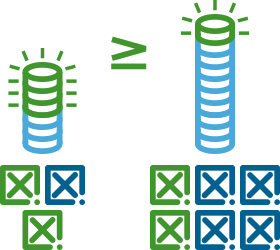
\includegraphics[height=2.5cm]{img/diminishingreturns}
		\end{subfigure}
	\end{figure}
\end{frame}





\subsection{Maximum Nash Social Welfare Problem}
\begin{frame}{Asymmetric Maximum Nash Social Welfare Problem}
	\pause
	\adjustfortopblock
	\begin{problem}<2->
		\begin{equation*}
			\alloc*[][] \overset{!}{=} \smashoperator{\argmax_{\alloc[][] \in \allallocs{\scriptstyle\agents\kern1pt}{\goods}}} \braces{ \NSW(\alloc[][]) }
			\onslide<4->{
				\qquad\text{with}\qquad
				\NSW(\alloc[][]) \coloneq \paren[\Big]{ \smashoperator{\prod_{i \in \agents}} \valuations[\alloc]^{\,\textstyle\weight} }{}^{\textstyle 1 / \sum_{i \in \agents} \weight}
			}
		\end{equation*}
		\begin{itemize}
			\item<2->
			\(\allallocs{\agents\kern1pt}{\goods}\): all possible allocations

			\item<3->
			\(\weight\): agent weight
		\end{itemize}
	\end{problem}
	\onslide<5->{The NSW strikes a middle ground between efficiency and fairness!}
	\begin{alertblock}<6->{}
		Is there a polynomial-time algorithm with an approximation factor \dots
		\begin{itemize}
			\item<8->
			\dots{} dependent on \(n\)?

			\item<9->
			\dots{} independent from \(m\)?
		\end{itemize}
		\def\svgwidth{3cm}
		\beamerimage<7-> at (13.5cm, 1.1cm) {\input{img/nvsm.pdf_tex}};
		\vspace{-0.75ex}
	\end{alertblock}
\end{frame}

	\section{RepReMatch}
\label{sec:reprematch}

\begin{algorithm*}[!b]
	\KwIn{%
		a set \(\goods\) of \(m\) items,
		a set \(\agents\) of \(n\) agents,
		submodular valuation functions \(\valuations \colon \powerset[\goods] \to \realposzero\) and weights \(\weight \in \realpos\) for all agents \(i \in \agents\)
	}
	\KwOut{%
		\(2n(\log_2 n + 3)\)-approximation \(\alloc[\phaseiii][] = (\alloc[\phaseiii])_{i \in \agents}\) of an optimal allocation
	}
	\phaseisep
	\(\alloc[\phasei] \gets \emptyset \quad\forall i \in \agents\)  \tct*{initialise temporary allocation}
	\(\goodsrem \gets \goods\)  \tct*{set of unassigned items}
	\For{\(t \gets 1, \dots, \ceil{\log_2 n}+1\)}{
		\If{\(\goodsrem \neq \emptyset\)}{
			\(\weights \gets \braces[\big]{\, \paren[\big]{ i, j, \weight \log{ \valuations[j] } } \given[\bigm] i \in \agents, j \in \goodsrem \,}\)   \tct*{weighted edges using val. of single item}
			\(\bipartitegraph \gets (\agents, \goodsrem, \weights)\)  \tct*{bipartite graph}
			\(\matching \gets \maxweightmatching(\bipartitegraph)\)\;
			\(\alloc[\phasei] \gets \alloc[\phasei] \cup \{j\} \quad \forall(i, j) \in \matching\)  \tct*{assign temporarily according to matching}
			\(\goodsrem \gets \goodsrem \setminus \{\, j \given (i, j) \in \matching \,\}\)  \tct*{remove assigned items}
		}
	}
	\phaseiisep
	\(\alloc[\phaseii] \gets \emptyset \quad\forall i \in \agents\)   \tct*{put allocation \(\alloc[\phasei][]\) away \& initialise new, definite one}
	\While{\(\goodsrem \neq \emptyset\)}{
		\(\weights \gets \braces[\big]{\, \paren[\big]{ i, j, \weight \log{ \valuations[ \alloc[\phaseii] \cup \{j\} ] } } \given[\bigm] i \in \agents, j \in \goodsrem \,}\)   \tct*{valuation of item \& current bundle}
		\(\bipartitegraph \gets (\agents, \goodsrem, \weights)\)\;
		\(\matching \gets \maxweightmatching(\bipartitegraph)\)\;
		\(\alloc[\phaseii] \gets \alloc[\phaseii] \cup \{j\} \quad \forall(i, j) \in \matching\)  \tct*{assign definitely according to matching}
		\(\goodsrem \gets \goodsrem \setminus \{\, j \given (i, j) \in \matching \,\}\)\;
	}
	\phaseiiisep
	\(\goodsrem \gets \bigcup_{i \in \agents} \alloc[\phasei]\)  \tct*{release items assigned in phase~\phasei} \label{ln:goodsrem}
	\(\weights \gets \braces[\big]{\, \paren[\big]{ i, j, \weight \log{ \valuations[ \alloc[\phaseii] \cup \{j\} ] } } \given[\bigm] i \in \agents, j \in \goodsrem \,}\)   \tct*{valuation of item \& current bundle}
	\(\bipartitegraph \gets (\agents, \goodsrem, \weights)\)\;
	\(\matching \gets \maxweightmatching(\bipartitegraph)\)\;
	\(\alloc[\phaseiii] \gets \alloc[\phaseii] \cup \{j\} \quad\forall(i, j) \in \matching\)  \tct*{initialise final allocation \& assign def. according to matching}
	\(\goodsrem \gets \goodsrem \setminus \{\, j \given (i, j) \in \matching \,\}\)\;
	\(\alloc[\phaseiii][] \gets \arballoc( \agents, \goodsrem, \alloc[\phaseiii][], (\valuations)_{i \in \agents} )\)  \tct*{assign remainder of items arbitrarily}
	\Return{\(\alloc[\phaseiii][]\)}
	\caption{%
		\RepReMatch{} for the asymmetric submodular \NSW{}
	}
	\label{alg:reprematch}
\end{algorithm*}

\subsection{Presentation of the Algorithm}
\label{subsec:reprematch:presentation}

The algorithm \SMatch{} estimates the valuation of the lowest-value items by determining the set of highest-value items and then valuing the remaining items.
Unfortunately, this approach does not work for general \emph{submodular} valuation functions because taking the set of highest-value items away does not necessarily leave a set of lowest-value items.
In fact, it can be shown \cite{submodular_low_value} that determining the set of lowest-value items is approximable only within a factor of \(\bigomega(\sqrt{m / \ln m})\).

For this reason, the algorithm \RepReMatch{} (\cref{alg:reprematch}) relies on an approach with three phases, thereby achieving an approximation factor of \(2n(\log_2 n + 3)\) (\cref{th:reprematch}).
In phase~\phasei, a sufficiently big set of high-value items is determined through repeated matchings.
This phase serves merley to determine this set, so items are assigned temporarily only.
The edge weights reflect this by taking the valuations of just single items into account.

In phase~\phaseii, the remaining items are assigned definitely through repeated matchings.
Consequently, each edge weight is updated in each round to be the weighted logarithm of the valuation of both the respective item and the items assigned so far.

In phase~\phaseiii, the high-value items assigned in phase \phasei{} are released.
With the knowledge of phase~\phaseii, one maximum weight matching is calculated, and the matched items are assigned accordingly.
Similarly to the previous phase, each edge weight is the weighted logarithm of the valuation of both the respective item and the respective agent's bundle from phase \phaseii.
The remaining released items are assigned arbitrarily.

\subsection{Analysis of the Algorithm}
\label{subsec:reprematch:analysis}

We use the term \emph{round} to refer to the iterations of the loops in the phases~\phasei{} and~\phaseii.
For ease of notation, we refer to the moment right before the first iteration in phase~\phaseii{} as round \(0\).
We start by analysing phase~\phaseii{} as it is the first phase with definitive assignments.
To this end, we introduce two types of item sets.
\begin{definition}
	Let \(\alloc*\) be an optimal bundle of an agent \(i \in \agents\).
	For any round \(r \ge 1\) in phase~\phaseii, the set \(\lostset{r} \subset \alloc*\) of \emph{lost items} is the set of all items \(j \in \alloc*\) assigned to other agents \(i' \neq i\) in that round.
\end{definition}
\begin{definition}
	Let \(\alloc*\) be an optimal bundle of an agent \(i \in \agents\) and \(\alloc[\phaseii] = \{ \asgd{1}, \dots, \asgd{\alloclen[\phaseii]} \}\) be her bundle at the end of phase \phaseii.
	The set of \emph{optimal and attainable items} is defined as \(\attopt{0} \coloneq \alloc* \setminus \bigcup_{i' \in \agents} \alloc[\phasei][i']\) for round~\(0\) and as \(\attopt{r} \coloneq \attopt{r-1} \setminus ( \lostset{r} \cup \{\asgd{r-1}\} )\) for round \(r = 1, \dots, \alloclen[\phaseii]\).
\end{definition}
\noindent
We denote their sizes by \(\lostsetlen{r}\ \coloneq \abs{\lostset{r}}\) and \(\attoptlen{r} \coloneq \abs{\attopt{r}}\), respectively.
First, we give a lower bound on the valuations of optimal and attainable items.
\begin{lemma}
	\label{lem:induction}
	For each agent \(i \in \agents\) and her bundle \(\alloc[\phaseii] = \{ \asgd{1}, \dots, \asgd{\alloclen[\phaseii]} \}\), it holds in all rounds \(r = 2, \dots, \alloclen[\phaseii]\) of phase \phaseii{} that
	\begin{equation*}
		\valuations[ \attopt{r} \given \asgd{1}, \dots, \asgd{r-1} ] \ge \valuations[\attopt{1}] - \smashoperator{\sum_{r'=1}^{r-1}} \lostsetlen{r'+1} \cdot \valuations[ \asgd{r'} \given \asgd{1}, \dots, \asgd{r'-1} ] - \valuations[\asgd{1}, \dots, \asgd{r-1}] \mperiod
	\end{equation*}
\end{lemma}
\begin{proof}
	The proof by \citeauthor{APNSWuSVþUM}~\cite[13\psq]{APNSWuSVþUM} consists of a lengthy induction rich in formulae and case differentiations.
	This is why we give a different but intuitive approach.

	Writing the left-hand side of the lemma out in full gives
	\begin{equation}
		\valuations[ \attopt{r} \given \asgd{1}, \dots, \asgd{r-1} ]
		= \valuations[ \attopt{r} \cup \braces{ \asgd{1}, \dots, \asgd{r-1} } ] - \valuations[ \asgd{1}, \dots, \asgd{r-1} ] \mperiod[,]
		\label{eq:attopt_marginal}
	\end{equation}
	which explains the second subtrahend on the right-hand side.

	Next, we show a lower bound on \(\valuations[\attopt{r} \cup \braces{ \asgd{1}, \dots, \asgd{r-1} }]\).
%	The set \(\attopt{r}\) of optimal and attainable items in round~\(r\) is equal to the set \(\attopt{r}\) of optimal and attainable items in round \(r-1\) minus the set \(\lostset{r}\) of lost items of round~\(r\) and, possibly, the item \(\asgd{r-1}\) assigned in round \(r-1\) if it was optimal back then, \ie, \(\asgd{r-1} \in \attopt{r-1}\).
	The items which are optimal and attainable in round \(r\) were so in round~\(r-1\), too.
	Additionally, the optimal but lost items of round \(r\) were attainable in round \(r-1\) as well.
	The item \(\asgd{r}\) assigned to agent \(i\) in round \(r\) was also attainable in round \(r-1\) and may also be optimal.
	Therefore, it holds \(\paren{ \attopt{r} \cup \braces{\asgd{r-1}} } \supset \paren{ \attopt{r-1} \setminus \lostset{r} }\) and
	\begin{equation}
		\valuations[\attopt{r} \cup \braces{ \asgd{1}, \dots, \asgd{r-1} }]
		\ge \valuations[\attopt{r-1} \setminus \lostset{r} \cup \braces{ \asgd{1}, \dots, \asgd{r-2} }]
		\ge \valuations[\attopt{r-1} \cup \braces{ \asgd{1}, \dots, \asgd{r-2} }] - \valuations[\lostset{r}] \mperiod
		\label{eq:attopt_union}
	\end{equation}
	The second inequality makes intuitively sense when one thinks of diminishing returns:
	The gain from adding the set \(\lostset{r}\) to the items in \(\attopt{r-1} \cup \braces{ \asgd{1}, \dots, \asgd{r-1} }\) cannot be higher than its subtracted valuation over the empty set.
	If we now recursively apply \cref{eq:attopt_union}, we eventually arrive at
	\begin{equation}
		\valuations[\attopt{r} \cup \braces{ \asgd{1}, \dots, \asgd{r-1} }]
		\ge \valuations[\attopt{1}] - \sum_{r'=1}^{r-1} \valuations[\lostset{r'+1}] \mperiod
		\label{eq:attop_lost}
	\end{equation}

	Lastly, we give an upper bound on \(\valuations[\lostset{r'+1}]\).
	The valuation \(\valuations[j \given \asgd{1}, \dots, \asgd{r'-1}]\) of any item \(j \in \lostset{r'+1}\) in round \(r'\) cannot have been higher than \(\valuations[\asgd{r'} \given \asgd{1}, \dots, \asgd{r'-1}]\) as otherwise item \(\asgd{r'}\) would not have been assigned before item \(j\).
	From this follows
	\begin{equation}
		\valuations[\lostset{r'+1}] \le \lostsetlen{r'+1} \cdot \valuations[\asgd{r'} \given \asgd{1}, \dots, \asgd{r'-1}] \mperiod
		\label{eq:lost}
	\end{equation}
	Combining \cref{eq:attopt_marginal,eq:attop_lost,eq:lost} proves the lemma.
\end{proof}
%\begin{lemma}
%	\label{lem:induction}
%	For each agent \(i \in \agents\) and her bundle \(\alloc[\phaseii] = \{ \asgd{1}, \dots, \asgd{\alloclen[\phaseii]} \}\), it holds in all rounds \(r = 2, \dots, \alloclen[\phaseii]\) of phase \phaseii{} that
%	\begin{equation*}
%		\valuations[ \attopt{r} \given \asgd{1}, \dots, \asgd{r-1} ] \ge \valuations[\attopt{1}] - \lostsetlen{2} \cdot \valuations[\asgd{1}] - \smashoperator{\sum_{r'=2}^{r-1}} \lostsetlen{r'+1} \cdot \valuations[ \asgd{r'} \given \asgd{1}, \dots, \asgd{r'-1} ] - \valuations[\asgd{1}, \dots, \asgd{r-1}] \mperiod
%	\end{equation*}
%\end{lemma}
%\begin{proof}
%	We prove the lemma by induction on the number \(r\) of rounds.
%	In the beginning of the base case \(r=2\), agent \(i\) has already been assigned item \(\asgd{1}\).
%	For each of the optimal and attainable items~\(j \in \attopt{1}\) in round \(1\), the marginal valuation \(\valuations[j \given \emptyset]\) over the empty set was at most \(\valuations[\asgd{1} \given \emptyset]\), as otherwise item~\(\asgd{1}\) would not have been assigned first.
%	The marginal valuation \(\valuations[j \given \asgd{1}]\) over \(\{\asgd{1}\}\) is upper-bounded by \(\valuations[\asgd{1} \given \emptyset]\), too, due to the submodularity of valuations.
%	During round \(2\), a further \(\lostsetlen{2}\) of these items \(j\) are assigned to other agents, and item \(\asgd{2}\) is assigned to agent \(i\).
%	We can bound the marginal valuation of the remaining optimal and attainable items in round \(2\) in the following way:
%	\begin{caseintext}{1}{\(\asgd{1} \in \attopt{1}\)}
%		It holds \(\valuations[ \attopt{2} \given \asgd{1} ] = \valuations[ \attopt{2} \cup \{\asgd{1}\} ] - \valuations[\asgd{1}] = \valuations[\attopt{1} \setminus \lostset{2}] -  \valuations[\asgd{1}]\).
%	\end{caseintext}
%	\begin{caseintext}{2}{\(\asgd{1} \notin \attopt{1}\)}
%		Due to the monotonicity of the valuation functions, it holds \(\valuations[ \attopt{2} \cup \{\asgd{1}\} ] \ge \valuations[ \attopt{2} ]\) and, therefore, \(\valuations[ \attopt{2} \given \asgd{1} ] \ge \valuations[ \attopt{2} ] - \valuations[\asgd{1}] = \valuations[\attopt{1} \setminus \lostset{2}] -  \valuations[\asgd{1}]\).
%	\end{caseintext}
%	\noindent
%	In both cases, the base case is proven because
%	\begin{equation}
%		\valuations[ \attopt{2} \given \asgd{1} ]
%		\ge \valuations[\attopt{1} \setminus \lostset{2}] -  \valuations[\asgd{1}]
%		\ge \valuations[ \attopt{1} ] - \valuations[\lostset{2}] - \valuations[\asgd{1}]
%		\ge \valuations[ \attopt{1} ] - \lostsetlen{2} \cdot \valuations[\asgd{1}] - \valuations[\asgd{1}] \mperiod[,]
%	\end{equation}
%	where the second inequality is shown easily using an alternative definition of submodularity (\(\valuations[\genericset[1] \cup \genericset[2]] + \valuations[\genericset[1] \cap \genericset[2]] \le \valuations[\genericset[1]] + \valuations[\genericset[2]]\) with \(\genericset[1] = \attopt{1} \setminus \lostset{2}\) and \(\genericset[2] = \lostset{2} \)~\cite{inapprox_results_for_combi_auctions_with_submod_utility_funcs}), and the third inequality is due to all \(\lostsetlen{2}\) items \(j\) in set \(\lostset{2}\) not being assigned in round \(1\) although attainable, implying \(\valuations[j] \le \valuations[\asgd{1}]\).
%
%	For the induction hypothesis, we assume that the lemma holds true for all rounds up to some~\(r\).
%	In the induction step \(r \to r+1\), we differentiate the same two cases again:
%	\begin{caseintext}{1}{\(\asgd{r} \in \attopt{r}\)}
%		Again we exploit the submodularity of the valuation functions to obtain a lower bound on the marginal valuation of \(\attopt{r+1}\).
%		\begin{align}
%			\valuations[ \attopt{r+1} \given \asgd{1}, \dots, \asgd{r} ]
%			&= \valuations[ \attopt{r+1} \cup \{\asgd{r}\} \given \asgd{1}, \dots, \asgd{r-1} ] - \valuations[ \asgd{r} \given \asgd{1}, \dots, \asgd{r-1} ] \\
%			&= \valuations[ \attopt{r} \setminus \lostset{r+1} \given \asgd{1}, \dots, \asgd{r-1} ] - \valuations[ \asgd{r} \given \asgd{1}, \dots, \asgd{r-1} ] \\
%			&\ge \valuations[ \attopt{r} \given \asgd{1}, \dots, \asgd{r-1} ] - \valuations[ \asgd{r} \given \asgd{1}, \dots, \asgd{r-1} ] - \valuations[ \lostset{r+1} \given \asgd{1}, \dots, \asgd{r-1} ]
%		\end{align}
%	\end{caseintext}
%	\begin{caseintext}{2}{\(\asgd{r} \notin \attopt{r}\)}
%		At first, we use the monotonicity of the valuation functions to get the inequality
%		\begin{align}
%			\valuations[ \attopt{r} \given \asgd{1}, \dots, \asgd{r} ]
%			&= \valuations[ \attopt{r} \cup \{ \asgd{1}, \dots, \asgd{r} \} ] - \valuations[\asgd{1}, \dots, \asgd{r}] \\
%			&\ge \valuations[ \attopt{r} \cup \{ \asgd{1}, \dots, \asgd{r-1} \} ] - \valuations[\asgd{1}, \dots, \asgd{r}] \\
%			&= \begin{multlined}[t]
%				\paren[\big]{ \valuations[ \attopt{r} \cup \{ \asgd{1}, \dots, \asgd{r-1} \} ] - \valuations[\asgd{1}, \dots, \asgd{r-1}] } \\
%				- \paren[\big]{ \valuations[\asgd{1}, \dots, \asgd{r}] - \valuations[\asgd{1}, \dots, \asgd{r-1}] }
%			\end{multlined} \\
%			&= \valuations[ \attopt{r} \given \asgd{1}, \dots, \asgd{r-1} ] - \valuations[ \asgd{r} \given \asgd{1}, \dots, \asgd{r-1} ] \mperiod
%		\end{align}
%		Together with the submodularity of valuation, we obtain the same lower bound again:
%		\begin{align}
%			\valuations[ \attopt{r+1} \given \asgd{1}, \dots, \asgd{r} ]
%			&= \valuations[ \attopt{r} \setminus \lostset{r+1} \given \asgd{1}, \dots, \asgd{r} ] \\
%			&\ge \valuations[ \attopt{r} \given \asgd{1}, \dots, \asgd{r} ] - \valuations[ \lostset{r+1} \given \asgd{1}, \dots, \asgd{r} ] \\
%			&\ge \valuations[ \attopt{r} \given \asgd{1}, \dots, \asgd{r} ] - \valuations[ \lostset{r+1} \given \asgd{1}, \dots, \asgd{r-1} ] \\
%			&\ge \valuations[ \attopt{r} \given \asgd{1}, \dots, \asgd{r-1} ] - \valuations[ \asgd{r} \given \asgd{1}, \dots, \asgd{r-1} ] - \valuations[ \lostset{r+1} \given \asgd{1}, \dots, \asgd{r-1} ]
%		\end{align}
%	\end{caseintext}
%	In both cases, we can replace \(\valuations[ \attopt{r} \given \asgd{1}, \dots, \asgd{r-1} ]\) by the induction hypothesis and \(\valuations[ \lostset{r+1} \given \asgd{1}, \dots, \asgd{r-1} ]\) by \(\lostsetlen{r+1} \cdot \valuations[ \asgd{r} \given \asgd{1}, \dots, \asgd{r-1} ]\) to prove the induction step.
%	\begin{align}
%		\valuations[ \attopt{r+1} \given \asgd{1}, \dots, \asgd{r} ]
%		&\ge \begin{multlined}[t]
%			\valuations[\attopt{1}] - \lostsetlen{2} \cdot \valuations[\asgd{1}] - \smashoperator{\sum_{r'=2}^{r-1}} \lostsetlen{r'+1} \cdot \valuations[ \asgd{r'} \given \asgd{1}, \dots, \asgd{r'-1} ] \\
%			- \valuations[\asgd{1}, \dots, \asgd{r-1}] - \valuations[ \asgd{r} \given \asgd{1}, \dots, \asgd{r-1} ] - \lostsetlen{r+1} \cdot \valuations[ \asgd{r} \given \asgd{1}, \dots, \asgd{r-1} ]
%		\end{multlined} \\
%		&= \valuations[\attopt{1}] - \lostsetlen{2} \cdot \valuations[\asgd{1}] - \smashoperator{\sum_{r'=2}^{r}} \lostsetlen{r'+1} \cdot \valuations[ \asgd{r'} \given \asgd{1}, \dots, \asgd{r'-1} ] - \valuations[\asgd{1}, \dots, \asgd{r}]
%	\end{align}
%\end{proof}

The lemma can be used to find a lower bound on the marginal valuation of the items actually assigned in each round \(r\).
\begin{corollary}
	\label{cor:lower_bound_single_item}
	From \cref{lem:induction} follows
	\begin{equation*}
		\valuations[ \asgd{r} \given \asgd{1}, \dots, \asgd{r-1} ]
		\ge \paren[\Big]{ \valuations[\attopt{1}] - \smashoperator{\sum_{r'=1}^{r-1}} \lostsetlen{r'+1} \cdot \valuations[ \asgd{r'} \given \asgd{1}, \dots, \asgd{r'-1} ] - \valuations[\asgd{1}, \dots, \asgd{r-1}] } \Big/ \attoptlen{r} \mperiod
	\end{equation*}
%	\begin{equation*}
%		\valuations[ \asgd{r} \given \asgd{1}, \dots, \asgd{r-1} ]
%		\ge \paren[\Big]{ \valuations[\attopt{1}] - \lostsetlen{2} \cdot \valuations[\asgd{1}] - \smashoperator{\sum_{r'=2}^{r-1}} \lostsetlen{r'+1} \cdot \valuations[ \asgd{r'} \given \asgd{1}, \dots, \asgd{r'-1} ] - \valuations[\asgd{1}, \dots, \asgd{r-1}] } \Big/ \attoptlen{r} \mperiod
%	\end{equation*}
\end{corollary}
\begin{proof}
%	There are \(\attoptlen{0}\) optimal and attainable items in \(\attopt{0}\) at the start of phase~\phaseii.
%	Of those, \(\lostsetlen{l}\) many are assigned to other agents in each round \(l \le r\), and also some items \(\asgd{l}\) assigned to agent \(i\) may be optimal, whence an upper bound of \(\attoptlen{0} - \sum_{l=1}^{r} \lostsetlen{l}\) on the number \(\attoptlen{r}\) of items in the set \(\attopt{r}\).\todo{Possibly this whole estimation can be omitted as we ditch it in the following lemma.}

	Remember that valuation functions are monotonic if \(\valuations[\genericset[1]] \le \valuations[\genericset[2]]\) holds for all sets \(\genericset[1] \subset \genericset[2] \subset \goods\).
	Induction shows that there must be an item \(j \in \genericset[2]\) with valuation \(\valuations[j] \ge \valuations[\genericset[2]] / \abs{\genericset[2]}\), otherwise it would hold \(\valuations[\emptyset] > 0\).
	Applied to \cref{lem:induction}, this means that there must be an item \(j \in \attopt{r}\) with a marginal valuation of at least \(\valuations[ \attopt{r} \given \asgd{1}, \dots, \asgd{r-1} ] / \attoptlen{r}\)\mperiod{}
	As item \(\asgd{r}\) was the one to be assigned, its marginal valuation cannot be smaller.
\end{proof}

This, finally, enables us to give a lower bound on the valuation of the bundles \(\alloc[\phaseii]\).
\begin{lemma}
	\label{lem:lower_bound_all_items}
	For each agent \(i \in \agents\) and her bundle \(\alloc[\phaseii] = \{\asgd{1}, \dots, \asgd{\alloclen[\phaseii]}\}\), it holds
	\begin{equation*}
		\valuations[\asgd{1}, \dots, \asgd{\alloclen[\phaseii]}] \ge \valuations[\attopt{1}] / n \mperiod
	\end{equation*}
\end{lemma}
\begin{proof}
	In each round \(r = 1, \dots, \alloclen[\phaseii]\), \(\lostsetlen{r}\) optimal and attainable items of agent \(i\) are assigned to other agents.
	As there are \(n\) agents in total, \(n-1\) is an upper bound on \(\lostsetlen{r}\).
	Furthermore, after \(\alloclen[\phaseii]\) rounds, the number \(\attoptlen{\alloclen[\phaseii]}\) of optimal and attainable items is at most \(n-1 \le n\) elsewise agent \(i\) would have been assigned yet another item.
	Together with \cref{cor:lower_bound_single_item}, this proves the lemma:
	\begin{align}
		\valuations[\asgd{1}, \dots, \asgd{\alloclen[\phaseii]}]
		&= \valuations[\asgd{1}, \dots, \asgd{\alloclen[\phaseii] - 1}] + \valuations[ \asgd{\alloclen[\phaseii]} \given \asgd{1}, \dots, \asgd{\alloclen[\phaseii]} ] \\
		&\ge \begin{multlined}[t]
			\valuations[\asgd{1}, \dots, \asgd{\alloclen[\phaseii] - 1}] + \paren[\Big]{ \valuations[\attopt{1}] - \smashoperator{\sum_{r'=1}^{\alloclen[\phaseii]-1 \mathstrut}} \lostsetlen{r'+1} \cdot \valuations[ \asgd{r'} \given \asgd{1}, \dots, \asgd{r'-1} ] \\
				- \valuations[\asgd{1}, \dots, \asgd{\alloclen[\phaseii]-1}] } \Big/ \attoptlen{\alloclen[\phaseii]}  % \Big/ has better spacing than \Bigm/.
		\end{multlined} \\
		&\ge \begin{multlined}[t]
			\valuations[\asgd{1}, \dots, \asgd{\alloclen[\phaseii] - 1}] + \paren[\Big]{ \valuations[\attopt{1}] - \smashoperator{\sum_{r'=1}^{\alloclen[\phaseii]-1 \mathstrut}} (n-1) \valuations[ \asgd{r'} \given \asgd{1}, \dots, \asgd{r'-1} ] \\
				- \valuations[\asgd{1}, \dots, \asgd{\alloclen[\phaseii]-1}] } \Big/ n
		\end{multlined} \\
		&\ge \valuations[\asgd{1}, \dots, \asgd{\alloclen[\phaseii] - 1}] + \paren[\big]{ \valuations[\attopt{1}] - (n-1) \valuations[\asgd{1}, \dots, \asgd{\alloclen[\phaseii]-1}] - \valuations[\asgd{1}, \dots, \asgd{\alloclen[\phaseii]-1}] } \big/ n \\
		&= \valuations[\attopt{1}] / n
	\end{align}
%	\begin{align}
%		\valuations[\asgd{1}, \dots, \asgd{\alloclen[\phaseii]}]
%		&= \valuations[\asgd{1}, \dots, \asgd{\alloclen[\phaseii] - 1}] + \valuations[ \asgd{\alloclen[\phaseii]} \given \asgd{1}, \dots, \asgd{\alloclen[\phaseii]} ] \\
%		&\ge \begin{multlined}[t]
%			\valuations[\asgd{1}, \dots, \asgd{\alloclen[\phaseii] - 1}] + \paren[\Big]{ \valuations[\attopt{1}] - \lostsetlen{2} \cdot \valuations[\asgd{1}] - \smashoperator{\sum_{r'=2}^{\alloclen[\phaseii]-1 \mathstrut}} \lostsetlen{r'+1} \cdot \valuations[ \asgd{r'} \given \asgd{1}, \dots, \asgd{r'-1} ] \\
%				- \valuations[\asgd{1}, \dots, \asgd{\alloclen[\phaseii]-1}] } \Big/ \attoptlen{\alloclen[\phaseii]}  % \Big/ has better spacing than \Bigm/.
%		\end{multlined} \\
%		&\ge \begin{multlined}[t]
%			\valuations[\asgd{1}, \dots, \asgd{\alloclen[\phaseii] - 1}] + \paren[\Big]{ \valuations[\attopt{1}] - (n-1) \valuations[\asgd{1}] - \smashoperator{\sum_{r'=2}^{\alloclen[\phaseii]-1 \mathstrut}} (n-1) \valuations[ \asgd{r'} \given \asgd{1}, \dots, \asgd{r'-1} ] \\
%				- \valuations[\asgd{1}, \dots, \asgd{\alloclen[\phaseii]-1}] } \Big/ n
%		\end{multlined} \\
%		&\ge \valuations[\asgd{1}, \dots, \asgd{\alloclen[\phaseii] - 1}] + \paren[\big]{ \valuations[\attopt{1}] - (n-1) \valuations[\asgd{1}, \dots, \asgd{\alloclen[\phaseii]-1}] - \valuations[\asgd{1}, \dots, \asgd{\alloclen[\phaseii]-1}] } \big/ n \\
%		&= \valuations[\attopt{1}] / n
%	\end{align}
\end{proof}

After having obtained a lower bound on the valuation of items assigned in phase~\phaseii, we need a lower bound for phase~\phaseiii{} as well.
Therefor we introduce a third type of item set.
\begin{definition}
	Let \(\alloc* = \{ \asgd*{1}, \dots, \asgd{\alloclen*}\}\) be an optimal bundle of some agent \(i \in \agents\).
	The set of \emph{overly good} items is defined as \(\overlygoodset \coloneq \{\, j \in \goods \given \valuations[j] \ge \valuations[\asgd*{1}] \,\}\).
\end{definition}

\begin{lemma}
	\label{lem:overly_good_matching}
	In phase~\phaseiii, there exists a matching such that each agent \(i \in \agents\) is matched to one of her overly good items in the set \(\bigcup_{i' \in \agents} \alloc[\phasei][i']\) of released items.
\end{lemma}
\begin{proof}
	If all items were matched in phase~\phasei, \ie, \(\bigcup_{i' \in \agents} \alloc[\phasei][i'] = \goods\), then all optimal items are released in phase~\phaseiii{} and each agent can be matched to one;
	the lemma is proven immediately.
	If not, imagine for some~\(t\) that only the items assigned in the first~\(t\) rounds of phase~\phasei{} were released.
%	Denote the set of released items by \(\goodsreleased{t}\).
	Now choose some matching \(\matching[t]\) with the following properties:
	\begin{enumerate}
		\item
		\label[property]{enum:matching:agent}
		If for an agent \(i\) all overly good items were amongst the released items,
%		\ie, \(\overlygoodset \subset \goodsreleased{t}\),
		she gets matched with an overly good item \(j \in \overlygoodset\).

		\item
		\label[property]{enum:matching:max}
		The number of agents matched with one of their overly good items is maximal amongst all matchings fulfilling \cref{enum:matching:agent}.
	\end{enumerate}
	\Cref{enum:matching:agent} is always satisfiable as the union of \(k\) many sets \(\overlygoodset\) contains \(k\) different items~\(\asgd*{1}\), which can be matched with agents \(i\).
	\Cref{enum:matching:max} leads to all agents being matched with an overly good item when \(t = \ceil{\log_2 n}+1\), \ie{} the number of rounds in phase~\phasei, whence the lemma follows.
	To prove this, we denote by \(\unluckyagents{t}\) the set of agents who are \emph{not} matched with one of their overly good items, and show by induction on \(t\) that it holds \(\abs{\unluckyagents{t}} \le n/2^t\).

	In the base case \(t=1\), none of the items are assigned initially.
	Denote by \(\unluckyagentsalgo{1}\) the number of agents who were not assigned an overly good item in the first round of phase~\phasei.
	If \(\unluckyagentsalgo{1} \le n/2\), then a matching \(\matching[1]\) obviously exists and the base case is immediately proven.
	Otherwise, all items from at least \(\unluckyagentsalgo{1}\) many sets \(\overlygoodset\) got assigned to someone.
	Again:
	Each set \(\overlygoodset\) contains the item \(\asgd*{1}\), so the union of these sets contains at least~\(\unluckyagentsalgo{1}\) items which can be matched with at least \(\unluckyagentsalgo{1}\) agents upon release.
	This then leaves at most~\(n-\alpha < n/2\) agents not matched with an overly good item.

	For the induction hypothesis, we assume that the statement holds true for all rounds up to some \(t\).
	In the induction step \(t \to t+1\), by \cref{enum:matching:agent}, there is at least one unassigned, overly good item in each set \(\overlygoodset[i']\) of all agents \(i' \in \unluckyagents{t}\) at the start of round \(t+1\).
	Analogously to the base case, for at least half of those agents \(i'\), these unassigned items will be assigned to either them or someone else, and it can be argued accordingly.
	By the induction hypothesis, it holds \(\abs{\unluckyagents{t+1}} \le \abs{\unluckyagents{t}}/2 \le (n/2^t)/2 = n/2^{t+1}\).
\end{proof}

This allows us to calculate an approximation factor for \RepReMatch{} by comparing its output with an optimal allocation \(\alloc*[][]\).
\begin{theorem}
	\label{th:reprematch}
	\RepReMatch{} has an approximation factor of \(2n (\log_2 n + 3)\).
\end{theorem}
\begin{proof}
	By \cref{lem:overly_good_matching}, we can assign each agent \(i\) an overly good item \(\overlygooditem \in \overlygoodset\) in the beginning of phase~\phaseiii.
	\RepReMatch{} maximises the logarithmic Nash social welfare, so
	\begin{equation}
		\label{eq:reprematch_approx_factor_lower_bound}
		\log \NSW(\alloc[\phaseiii][])
		\ge \frac{1}{\sum_{i \in \agents} \weight} \cdot \sum_{i \in \agents} \weight \log \valuations[\overlygooditem, \asgd{1}, \dots, \asgd{\alloclen[\phaseii]}]
	\end{equation}
	is a lower bound on the logarithmic \NSW{} after the first matching in phase~\phaseiii, with \(\alloc[\phaseii] = \{ \asgd{1}, \dots, \allowbreak \asgd{\alloclen[\phaseii]} \}\) being the bundle of agent \(i\) at the end of phase~\phaseii.

	Item \(\overlygooditem\) was released in phase~\phaseiii, which means it was assigned in phase~\phasei, implying \(\overlygooditem \in \alloc* \setminus \attopt{0}\) and, subsequently, \(\overlygooditem \in (\alloc* \setminus \attopt{0}) \cup \lostset{1}\).
	Phase~\phasei{} runs for at most \(\ceil{\log_2 n}+1\) rounds, and at most~\(n\) items are assigned in each iteration.
	Therefore, at most \(n (\log_2 n + 2)\) optimal items are assigned in that phase, \ie, \(\abs{ \alloc* \setminus \attopt{0} } \le n (\log_2 n + 2)\).
	As in \cref{lem:lower_bound_all_items}, it also holds \(n \ge \lostsetlen{1} = \abs{\lostset{1}}\).
	Together with the monotonicity of the valuation functions, this yields
	\begin{equation}
		\label{eq:overly_good_item_lower_bound}
		\valuations[ \overlygooditem, \asgd{1}, \dots, \asgd{\alloclen[\phaseii]} ]
		\ge \valuations[\overlygooditem]
		\ge \frac{\valuations[ (\alloc* \setminus \attopt{0}) \cup \lostset{1} ][\big]}{n(\log_2 n + 3)}
	\end{equation}
	as lower bound on the valuations of bundles.
	Moreover, \cref{lem:lower_bound_later_items} and the monotonicity of the valuation functions functions yield
	\begin{equation}
		\label{eq:assigned_items_lower_bound}
		\valuations[ \overlygooditem, \asgd{1}, \dots, \asgd{\alloclen[\phaseii]} ]
		\ge \valuations[ \asgd{1}, \dots, \asgd{\alloclen[\phaseii]} ]
		\ge \frac{\valuations[\attopt{1}]}{n}
		\ge \frac{\valuations[\attopt{1}]}{n(\log_2 n + 3)}
		= \frac{\valuations[ \attopt{0} \setminus \lostset{1} ]}{n(\log_2 n + 3)}
	\end{equation}
	as yet another lower bound.
	The mean of \crefrange{eq:overly_good_item_lower_bound}{eq:assigned_items_lower_bound} and the monotonicity of the valuation functions give the concise lower bound
	\begin{align}
		\valuations[ \overlygooditem, \asgd{1}, \dots, \asgd{\alloclen[\phaseii]} ]
		&\ge \frac{1}{2} \paren*{ \frac{\valuations[ (\alloc* \setminus \attopt{0}) \cup \lostset{1} ][\big]}{n(\log_2 n + 3)} + \frac{\valuations[ \attopt{0} \setminus \lostset{1} ][\big]}{n(\log_2 n + 3)} } \\
		&\ge \frac{1}{2} \cdot \frac{ \valuations[ \paren{(\alloc* \setminus \attopt{0}) \cup \lostset{1}} \cup \paren{\attopt{0} \setminus \lostset{1}} ][\big] }{n(\log_2 n + 3)} \\
		&= \frac{ \valuations[\alloc*] }{2n(\log_2 n + 3)} \mperiod
	\end{align}
	We can insert this lower bound into \cref{eq:reprematch_approx_factor_lower_bound} and prove the theorem thereby:
	\begin{equation}
		\log \NSW(\alloc[\phaseiii][])
		\ge \frac{1}{\sum_{i \in \agents} \weight} \cdot \sum_{i \in \agents} \weight \log \paren[\bigg]{ \frac{ \valuations[\alloc*] }{2n(\log_2 n + 3)} }
		= \log \paren[\bigg]{ \frac{\NSW(\alloc*[][])}{2n(\log_2 n + 3)} }
	\end{equation}
\end{proof}

\todo[inline]{overly good → outstanding?}

	\section{Conclusion}

\begin{frame}{Summary \& Outlook}
	\adjustfortopitem
	\begin{itemize}
		\item
		allocation:
		partition of items amongst agents

		\item
		bundles valued using submodular valuation functions
		\begin{itemize}
			\item
			diminishing returns
		\end{itemize}

		\item
		Nash social welfare:
		weighted geometric mean of valuations

		\item
		approximation factor independent from \(m\)?

		\item
		simple, repeated matching fails because of missing foresight

		\item
		\RepReMatch:
		\(2n (\log n + 3)\)-approximative
		\begin{description}
			\item[Phase \phasei]
			finding enough outstanding items

			\item[Phase \phaseii]
			assigning remaining item

			\item[Phase \phaseiii]
			assigning outstanding items
		\end{description}
	\end{itemize}
	\beamerimage at (13cm, 5.50cm) {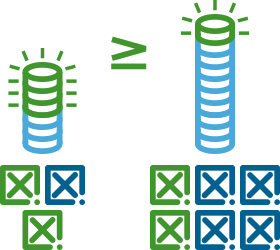
\includegraphics[height=1.45cm]{img/diminishingreturns}};
	\beamerimage at (13cm, 3.75cm) {
\includegraphics[height=1.45cm]{img/nvsm}};
	\beamerimage at (13cm, 2.00cm) {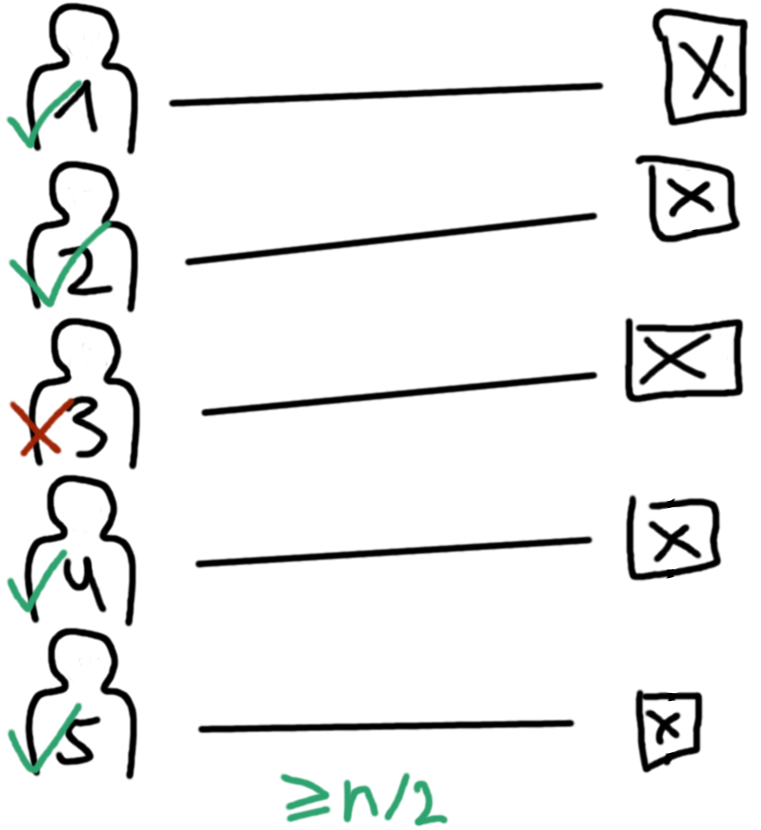
\includegraphics[height=1.45cm]{img/outstanding_1}};
	\beamerimage at (13cm, 0.25cm) {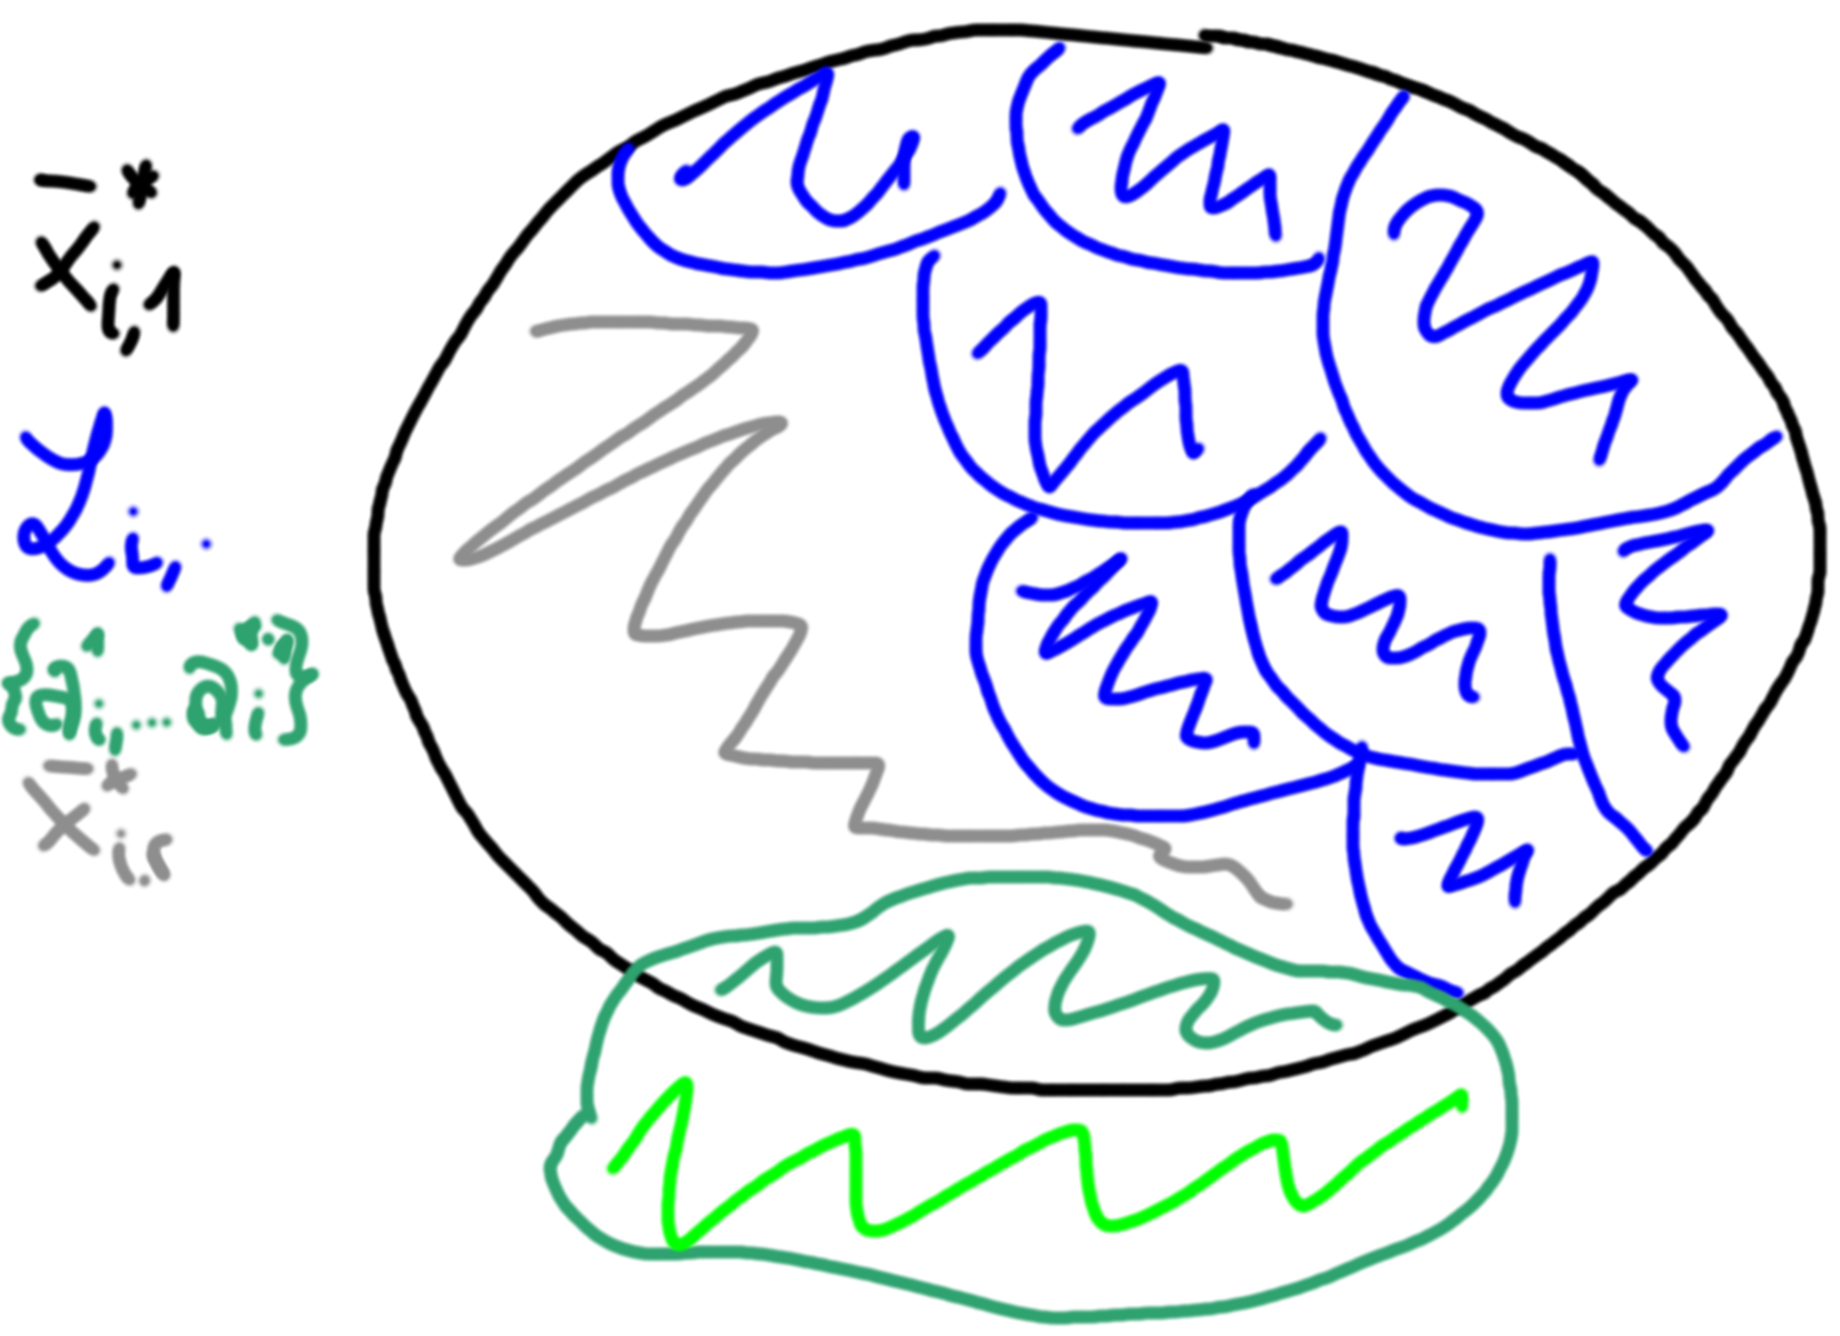
\includegraphics[height=1.45cm]{img/anal2_1}};
	\begin{minipage}{0.66\textwidth}
		\begin{block}{Any Room for Improvement?}
			Possibly! Lower bound of \(1.72\).
		\end{block}
	\end{minipage}
\end{frame}





\begin{frame}[c, plain, noframenumbering]
	\renewcommand{\insertsectionnumber}{!}
	\renewcommand{\insertsection}{End of Talk}
	\sectionpage
\end{frame}
\end{document}